\documentclass[border=10pt]{standalone}

\usepackage{tikz}
\usepackage{tikzsymbols}
\usetikzlibrary{calc,patterns,shapes.geometric}

\def\centerarc[#1](#2)(#3:#4:#5){\draw[#1] ($(#2)+({#5*cos(#3)},{#5*sin(#3)})$) arc (#3:#4:#5);}

\begin{document}
	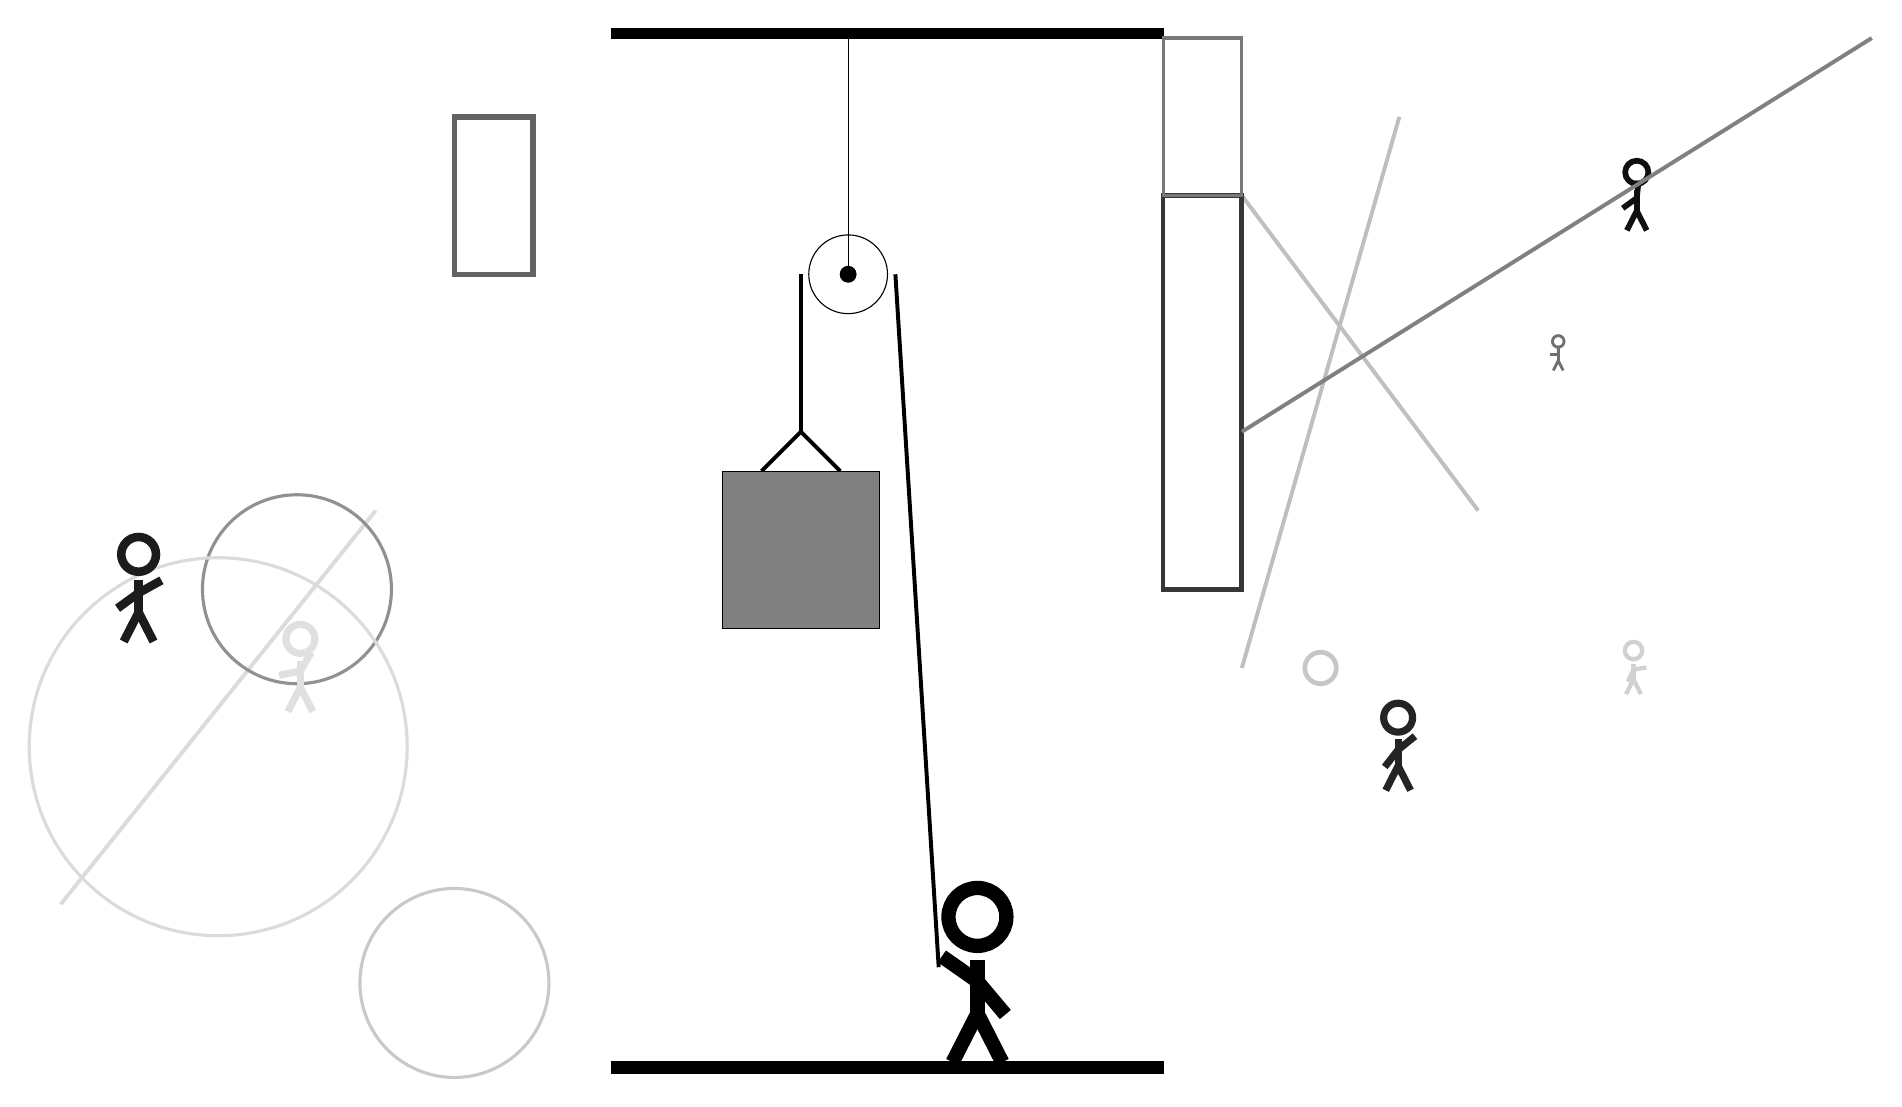
\begin{tikzpicture}
		%%%%% START %%%%%
		
		\draw[fill=black] (-2, 10) rectangle (5, 10.125);
		
		\draw (1, 7) circle (0.5);
		\draw[fill=black] (1, 7) circle (0.1);
		\draw (1, 10) -- (1, 7);
		
		\draw[line width=0.5mm, color=black!25](6, 8) -- (9, 4);
		
		\draw[line width=0.5mm, color=black!14](-5, 4) -- (-9, -1);
		\draw [line width=0.4mm, color=black!43](-6, 3) circle (1.2);
		\node[line width=0.6mm, color=black!86] at (8, 1) {\Strichmaxerl[5][52][39]};
		
		\draw [line width=0.4mm, color=black!14](-7, 1) circle (2.4);
		
		\node[line width=0.4mm, color=black!18] at (11, 2) {\Strichmaxerl[3][64][11]};
		\draw [line width=0.4mm, color=black!21](-4, -2) circle (1.2);
		
		\node[line width=0.5mm, color=black!94] at (11, 8) {\Strichmaxerl[4][36][84]};
		\draw[line width=0.5mm, color=black!25](8, 9) -- (6, 2);
		\node[line width=0.4mm, color=black!56] at (10, 6) {\Strichmaxerl[2][0][89]};
		\draw[line width=0.6mm, color=black!79] (6, 8) rectangle (5, 3);
		
		\draw [line width=0.6mm, color=black!22](7, 2) circle (0.2);
		\draw[line width=0.5mm, color=black!50](6, 5) -- (14, 10);
		\node[line width=0.2mm, color=black!12] at (-6, 2) {\Strichmaxerl[5][11][60]};
		\node[line width=0.2mm, color=black!89] at (-8, 3) {\Strichmaxerl[6][36][29]};
		\draw[line width=0.4mm, color=black!53] (6, 8) rectangle (5, 10);
		
		\draw[line width=0.7mm, color=black!61] (-3, 7) rectangle (-4, 9);
		
		\draw[line width=0.4mm, color=black!71] (5, 0) rectangle (5, 0);
		
		\draw[line width=0.5mm] (-0.1, 4.5) -- (0.4, 5.0) -- (0.9, 4.5);
		\draw[fill=black!50] (-0.6, 4.5) rectangle (1.4, 2.5);
		
		\draw[line width=0.5mm] (0.4, 7) -- (0.4, 5.0);
		\centerarc[line width=0.5mm](1, 7)(0:180:0.6);
		\draw[line width=0.5mm](1.6, 7) -- (2.15, -1.8);
		
		\node at (2.6, -1.9) {\Strichmaxerl[10][-35][-50]};
		
		\draw[fill=black] (-2, -3) rectangle (5, -3.15);
		
		%%%%% END %%%%%
	\end{tikzpicture}
\end{document}